\documentclass[a4paper,12pt]{article}
\usepackage{luatexja}
\usepackage{luatexja-fontspec}
\usepackage{geometry}
\usepackage{multicol}
\usepackage{titlesec}
\usepackage{setspace}
\usepackage{graphicx}
\usepackage{caption}
\usepackage{indentfirst}
\usepackage{float} % 図の位置を制御するために追加
\usepackage[utf8]{inputenc}
\usepackage{listings}
\usepackage{xcolor}

\geometry{margin=1in}

% 図のキャプションの表記を「図1」のように日本語化
\renewcommand{\figurename}{図}
\captionsetup[figure]{labelformat=default,labelsep=period}

\geometry{margin=25mm}
\setstretch{1.2}
\parindent=2em

\titleformat{\section}{\large\bfseries}{\thesection.}{1em}{}

\definecolor{keywordcolor}{rgb}{0.26, 0.38, 0.68}
\definecolor{commentcolor}{rgb}{0.3, 0.6, 0.3}
\definecolor{stringcolor}{rgb}{0.7, 0.2, 0.2}

\lstdefinelanguage{SystemVerilog}{
  morekeywords={module,endmodule,input,output,logic,always_ff,if,else,begin,end,posedge,negedge},
  sensitive=true,
  morecomment=[l]{//},
  morecomment=[s]{/*}{*/},
  morestring=[b]",
}

\lstset{
  language=SystemVerilog,
  basicstyle=\ttfamily\small,
  keywordstyle=\color{keywordcolor}\bfseries,
  commentstyle=\color{commentcolor}\itshape,
  stringstyle=\color{stringcolor},
  numbers=left,
  numberstyle=\tiny,
  stepnumber=1,
  numbersep=5pt,
  frame=single,
  tabsize=2,
  showstringspaces=false,
  breaklines=true,
  breakatwhitespace=true
}

\title{SystemVerilog Code with Listings}

\begin{document}

% タイトルブロック
\begin{center}
\noindent
{\LARGE 第1回輪講資料} \\
{\large 4321 野秋 琳太郎} \\
2025年 5月 23日
\end{center}

\begin{flushright}
指導教員 宮田 尚起
\end{flushright}

% 二段組開始
\begin{multicols}{2}

\section{はじめに}
LEDで光通信をして,「糸なし糸電話」をやりたい.
産技祭にだして,稲毛研究室と距離で競いたい.

\section{方針}
図\ref{fig:block}のような構成で通信を行うことにした.
LEDの照度でアナログなデータを送るのは難しいと考えたので,LEDの点灯/消灯でデジタルなデータを送ることにした.\\
 デジタル通信にはUARTを使用する.
信号線が1本でよく,TeraTermなどを利用すればデバッグも容易なためである.
midiなど,音を送る通信での採用例もある.\\
 ここで,光通信はホトカップラとして見做すことができる.
よって,受信側は入力のアナログ信号をUARTで送信,送信側は受信したUARTをD-Aコンバータからアナログ信号として出力というように,適当なライブラリを利用すれば簡単に実装できる.

\begin{figure}[H] % [H]で強制的にここに図を表示
  \centering
  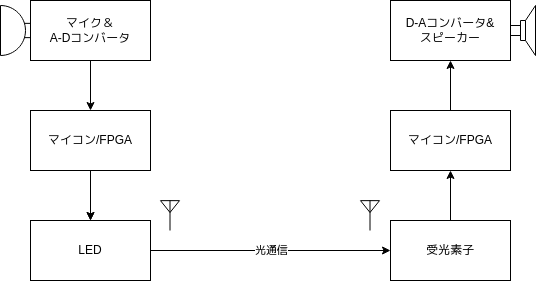
\includegraphics[width=\linewidth]{block.drawio.png}
  \caption{光通信のブロック図}
  \label{fig:block}
\end{figure}

\section{分担}
班で役割分担をした.
その内容は以下のとおりである.
輪講では,自分の分だけ進捗を発表する.

\begin{itemize}
\item
  瀬田:オーディオ入力,A-D変換
\item
  本橋:LEDを駆動
\item
  林 :LED,アンテナ
\item
  野秋:UART受信,D-A変換,オーディオ出力
\end{itemize}

\section{製作}
UARTの受信,D-A変換,オーディオ出力には図\ref{fig:fpga}にあるFPGA,Tang Primer 20kを使用する.
図\ref{fig:audio}に示すとおり,Tang Primer 20k のDockにはDACとアンプがついており,外付けの回路を作らずにD-A変換,オーディオ出力ができる.
よって,FPGAで作るべき回路はUART受信,DAC用のインターフェースである.
今週はUARTの送受信回路をSystem Verilogで書いた.
1文字の入出力ができることを確認してある.

\begin{figure}[H] % [H]で強制的にここに図を表示
  \centering
  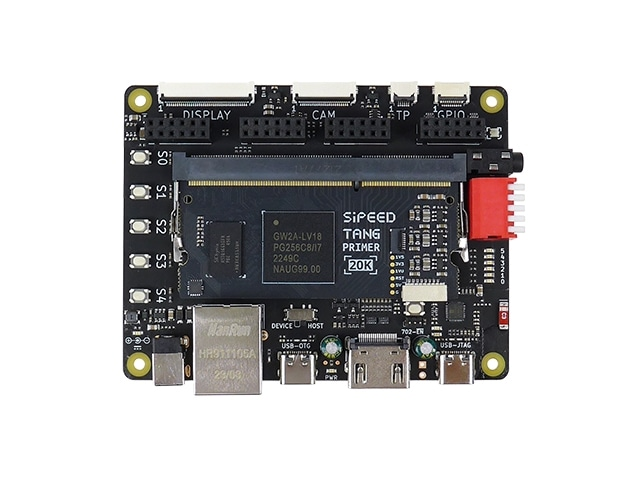
\includegraphics[width=\linewidth]{fpga.jpg}
  \caption{Tang Primer 20k}
  \label{fig:fpga}
\end{figure}

\end{multicols}

\begin{figure}[H] % [H]で強制的にここに図を表示
  \centering
  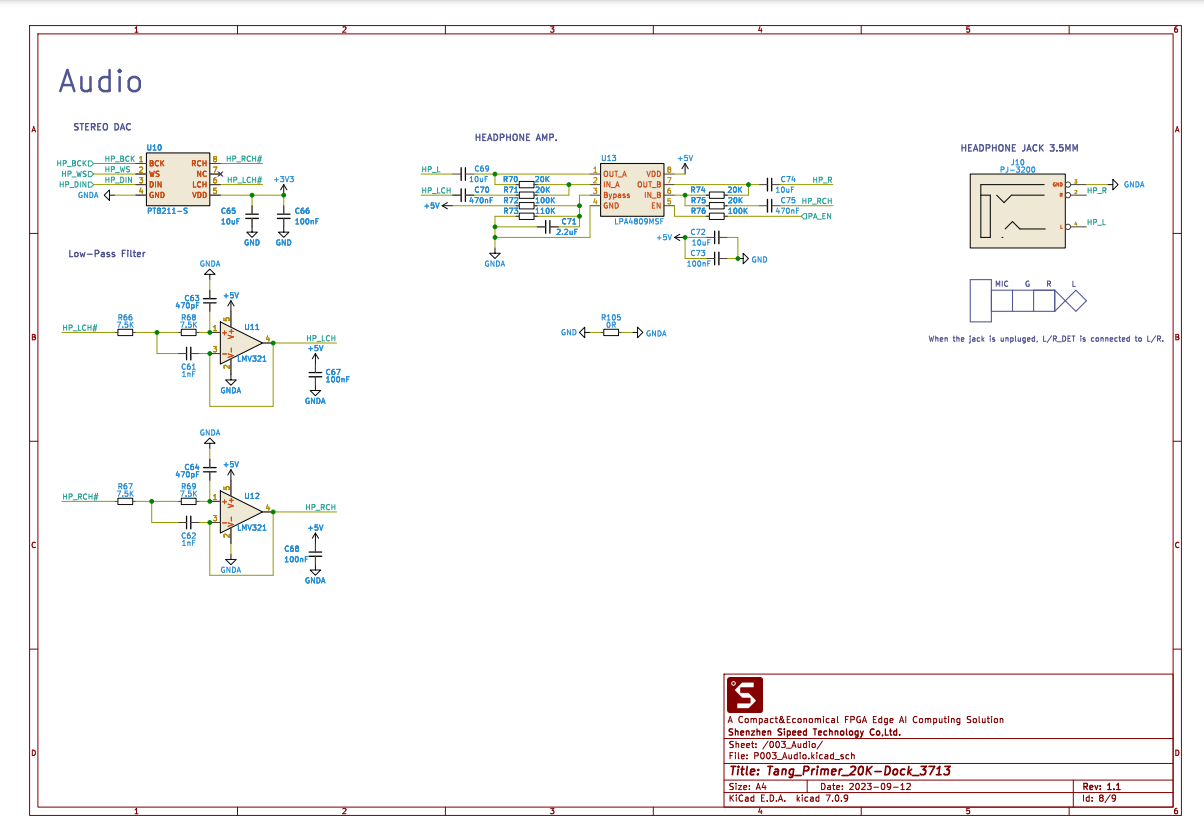
\includegraphics[width=\linewidth]{audio.png}
  \caption{オーディオ入出力}
  \label{fig:audio}
\end{figure}


\begin{lstlisting}
module uart(
    input clock,
    input reset,
    input RxD,
    input [7:0] Tx_buffer,
    input enable_trig,
    output logic TxD,
    output logic [7:0] Rx_buffer
);
//FPGAのクロック周波数/ボーレイト
parameter baud_div=27000000/115200;
//信号のハラのぶぶん
parameter valid=baud_div/2;

//マシンのステート
typedef enum logic [2:0]{
idle=3'b000,
strt=3'b001,
trns=3'b010,
mrgn=3'b011,
stop=3'b100
} uart_state;

//Tx_baud gen
reg [11:0]Tx_counter;
wire Tx_trig;
//uart Tx
uart_state Tx_state;
logic [2:0]Tx_bit_counter;

//Rx_baud gen
reg [11:0]Rx_counter;
wire Rx_trig;
wire Rx_valid;
//Rx_strt
logic Rx_prev;
wire  Rx_strt;
//uart Rx
uart_state Rx_state;
logic [2:0]Rx_bit_counter;

//Tx_baud gen
always @(posedge clock or negedge reset) begin
    if(!reset)Tx_counter<=0;
    else begin
        Tx_counter<=(baud_div==Tx_counter)?(1'b0):(Tx_counter+1'b1);
        if(!enable_trig) Tx_counter<=0;
    end
end

assign Tx_trig=(baud_div==Tx_counter)?(1):(0);

//uart Tx
always @(posedge clock or negedge reset) begin
    if(!reset)begin
        Tx_state<=idle;
        Tx_bit_counter<=0;
        TxD<=1;
    end
    else begin
        case(Tx_state)
            idle:begin
                TxD<=1;
                if(!enable_trig)Tx_state<=strt;
            end
            strt:begin
                TxD<=0;
                if(Tx_trig)begin
                    Tx_state<=trns;
                    Tx_bit_counter<=0;
                end
            end
            trns:begin
                TxD<=Tx_buffer[Tx_bit_counter];
                if(Tx_trig)begin
                    Tx_bit_counter<=Tx_bit_counter+1'b1;
                    if(Tx_bit_counter==3'b111) Tx_state<=stop;
                end
            end
            stop:begin
                TxD<=1;
                if(Tx_trig)Tx_state<=idle;
            end
        endcase
    end
end

//Rx_baud gen
//Rx_trig,Rx_valid
always @(posedge clock or negedge reset) begin
    if(!reset)Rx_counter<=0;
    else Rx_counter<=(Rx_strt==1 || baud_div==Rx_counter)?(1'b0):(Rx_counter+1'b1);
end

assign Rx_trig=(baud_div==Rx_counter)?(1):(0);
assign Rx_valid=(valid==Rx_counter)?(1):(0);

//Rx_strt
always@(posedge clock or negedge reset)begin
    if(!reset) Rx_prev<=1;
    else Rx_prev<=RxD;
end

//待機状態で,Rxの立下りエッジにいるときRx_strt=1
assign Rx_strt=(Rx_state==idle && Rx_prev==1 && RxD==0)?(1):(0);

//uart Rx
always @(posedge clock or negedge reset) begin
    if(!reset)begin
        Rx_state<=idle;
        Rx_buffer<=0;
    end
    else begin
        case(Rx_state)
            idle:if(Rx_strt)Rx_state<=strt;
            strt:begin
                if(Rx_trig)begin
                    Rx_state<=trns;
                    Rx_bit_counter<=0;
            end
            end
            trns:begin
                //7はマジックナンバー,よくない
                if(Rx_valid)begin
                    Rx_buffer[Rx_bit_counter]<=RxD;
                    Rx_bit_counter<=Rx_bit_counter+1'b1;
                    if(Rx_bit_counter==7) Rx_state<=mrgn;
                end
            end
            mrgn:if(Rx_trig)Rx_state<=stop;
            stop:if(Rx_trig)Rx_state<=idle;
        endcase
    end
end
endmodule
\end{lstlisting}

\section{今後の定}
\begin{multicols}{2}
D-Aコンバータのインターフェースを作って,手元で確認ができるようにする.
\end{multicols}


\end{document}
